\chapter{Inflation, Structure, and the Fate of Initial Conditions}

These notes follow Leonard Susskind's eighth lecture on cosmology, with the line of argument and the surviving board evidence preserved from the classroom record prepared through LazyingArt LLC and Video2Book. The lecture begins with a student's question about \(\Omega\), turns that question into an observational statement about the flatness of the universe, and then asks what mechanism could make the universe so large, so smooth, and yet not too smooth. Inflation is the proposed answer, but it becomes convincing only after we understand three linked points: why structure formation is delicate, why a slowly rolling scalar field can imitate vacuum energy, and why quantum fluctuations survive the very expansion that seems at first to erase them.

\section{Omega, Vacuum Energy, and the Evidence for Flatness}

The lecture opens in a deliberately pedestrian way: what is \(\Omega\)? The point is not only to define a symbol, but to remind ourselves how the expansion equation is organized in the late universe. We are to think about an era well after radiation domination, including the present epoch, so the right-hand side contains vacuum energy, ordinary matter, dark matter, and curvature, while radiation may be neglected to a good approximation.

In that regime the Friedmann equation is written schematically as
\begin{equation}
H^2=\left(\frac{\dot a}{a}\right)^2=\frac{8\pi G}{3}\,(\rho_0+\rho_m)-\frac{k}{a^2},
\end{equation}
where \(\rho_0\) is the vacuum-energy density and \(\rho_m\) is the nonrelativistic matter density. The lecture emphasizes the contrast in how these pieces scale:
\begin{equation}
\rho_0=\text{constant},
\qquad
\rho_m=\frac{M}{a^3}.
\end{equation}
Vacuum energy does not dilute when the universe expands; matter does.

The early algebra on the board is somewhat garbled in the transcript, so for the normalized quantities it is better to write the standard cleaned form explicitly. Dividing the Friedmann equation by \(H^2\) leads to the density parameters
\begin{equation}
\Omega_\Lambda=\frac{8\pi G\,\rho_0}{3H^2},
\qquad
\Omega_m=\frac{8\pi G\,\rho_m}{3H^2},
\qquad
\Omega_k=-\frac{k}{a^2H^2},
\end{equation}
so that
\begin{equation}
\Omega_\Lambda+\Omega_m+\Omega_k=1.
\end{equation}
If space is exactly flat, \(k=0\), and therefore
\begin{equation}
\Omega_\Lambda+\Omega_m=1.
\end{equation}

This is the sense in which \(\Omega\) is a bookkeeping device: after normalizing by the observed \(H^2\), the various terms become fractions of the expansion budget. Matter here includes dark matter. Radiation could also be included, but in the present universe its contribution is negligible compared with matter and vacuum energy.

What makes this more than notation is the observational logic. One measures matter, including the dark matter inferred gravitationally; one measures the Hubble expansion; one independently measures curvature geometrically. If the sum of the normalized matter and vacuum pieces comes out close to one, that is evidence for flatness. Conversely, if the curvature is measured to be very close to zero, then the matter density determines what the vacuum contribution must be.

That is the first important rhythm of the lecture. The flatness of the universe is not introduced as a theoretical prejudice. It is presented as an empirical fact, checked in more than one way. The measured matter content, the Hubble expansion, and the geometry of large-scale space all point in the same direction: the universe is flat to within a few percent. The additional observation that the expansion tends toward an exponential law,
\begin{equation}
a(t)\propto e^{Ht},
\end{equation}
is then taken as direct evidence that a vacuum-like component is present.

\section{Why Flatness Is Not Enough: The Need for Structure}

Having established that space is very nearly flat, Susskind immediately asks the next question: why is it so flat? His answer is inflation. To say that the universe is flat on very large scales is, in his language, to say that it is very big, very smooth, and very homogeneous. Inflation is the conjectured early period of exponential expansion that stretches the universe into that state.

But then comes the first deliberate reversal. One can overdo a good thing. If the universe were perfectly smooth, it would remain perfectly smooth. Gravity does not manufacture lumpiness out of exact symmetry. Galaxies, stars, and all later structure require primordial departures from homogeneity.

Tracing present structure backward, the lecture puts the inhomogeneity at the time of transparency, or just before it, at roughly one part in \(10^5\):
\begin{equation}
\frac{\delta\rho}{\rho}\sim 10^{-5}.
\end{equation}
This is small enough for the early universe to be extremely smooth, and yet large enough to act as a seed.

The mechanism is gravitational instability. A slight overdensity attracts matter from its surroundings. That increases the overdensity and deepens the neighboring underdensity. Unlike an ordinary gas in a room, which relaxes back to homogeneity under pressure and thermalization, self-gravitating matter amplifies its own irregularities.

\begin{figure}[t]
\centering
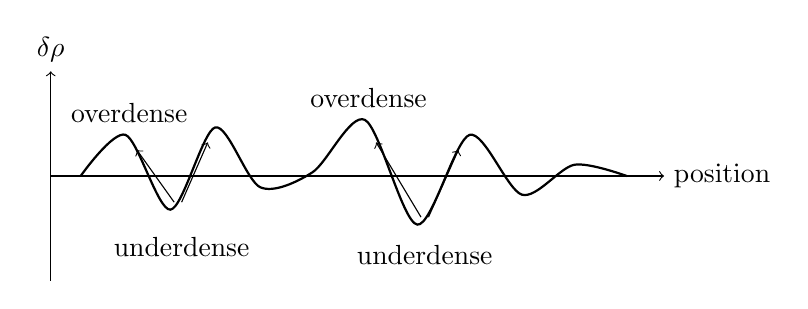
\begin{tikzpicture}[scale=0.95]
\draw[->] (0,-1.4) -- (0,1.4) node[above] {\(\delta\rho\)};
\draw[->] (0,0) -- (8.2,0) node[right] {position};
\draw[thick] plot[smooth] coordinates {
(0.4,0.0) (1.0,0.55) (1.6,-0.45) (2.2,0.65)
(2.8,-0.15) (3.5,0.05) (4.2,0.75) (4.9,-0.65)
(5.6,0.55) (6.3,-0.25) (7.0,0.15) (7.7,0.0)
};
\draw[->] (1.65,-0.35) -- (1.15,0.35);
\draw[->] (1.75,-0.35) -- (2.1,0.45);
\draw[->] (4.95,-0.55) -- (4.35,0.45);
\draw[->] (5.05,-0.55) -- (5.45,0.35);
\node at (1.05,0.85) {overdense};
\node at (4.25,1.05) {overdense};
\node at (1.75,-0.95) {underdense};
\node at (5.0,-1.05) {underdense};
\end{tikzpicture}
\caption{A schematic version of the lecture's structure-formation story: tiny overdensities pull matter out of neighboring underdense regions, so the contrast grows rather than relaxes away.}
\end{figure}

The lecture briefly reminds us that what is directly seen on the sky is not density itself but temperature anisotropy in the cosmic microwave background. Overdense regions look slightly colder because photons lose a bit more energy climbing out of deeper gravitational wells; on top of that there are Doppler contributions from the motion of the gas. The detailed mapping from primordial perturbations to the microwave background is complicated, but the bottom line is simple: by the time the universe became transparent, there were already fluctuations at the \(10^{-5}\) level.

\section{Pressure, Matter Domination, and the Onset of Collapse}

The next question comes naturally: if gravity amplifies overdensities, why did collapse not begin immediately? The answer is pressure. The lecture returns to the equation-of-state form
\begin{equation}
p=w\rho,
\end{equation}
and recalls the characteristic values
\begin{equation}
w_{\rm rad}=\frac13,
\qquad
w_m=0,
\qquad
w_{\rm vac}=-1.
\end{equation}

Radiation has positive pressure, and positive pressure tends to homogenize. That is why an ordinary gas in a room does not spontaneously clump into one corner. Matter, by contrast, is pressureless in the cosmological approximation. If there were no pressure at all and no gravity, an inhomogeneity would simply remain frozen in place. But once gravity is added, there is no pressure support to resist collapse, so the overdensity can grow.

During the radiation-dominated era the pressure was large enough to prevent gravity from forming lumps. Only when radiation became dynamically unimportant did gravity begin to win. In the lecture's language, one has a competition:
\begin{equation}
\text{gravity} \quad \text{versus} \quad \text{pressure}.
\end{equation}
While pressure dominates, structure is suppressed; once gravity dominates, contraction starts.

Dark matter enters here in a decisive way. It is the dark matter fluctuations that first begin to form large halos. Ordinary baryonic matter then falls into those potential wells, but unlike dark matter it does need dissipative processes in order to settle near the center and make luminous galaxies. Dark matter remains extended; baryonic matter can cool and condense.

There is also an important timing point. The epoch when matter overtook radiation dynamically is not exactly the same as the later epoch when the universe became transparent and atoms formed. The lecture places the onset of dark-matter contraction somewhat earlier, perhaps by a factor of ten in time, so that the first stages of the collapse are already underway before we can directly see back to the surface of last scattering.

\subsection{Question \& Answer}

\paragraph{Why didn't gravity make galaxies earlier?}

Because earlier on the universe was radiation dominated, and radiation carries positive pressure. In a radiation bath one has \(p=\rho/3\), and that pressure smooths irregularities instead of letting them implode. Only after matter became more important than radiation did pressure cease to block gravitational collapse.

Dark matter could begin this process slightly before ordinary matter. It was already present, effectively cold, and it could build large halos without first radiating away energy in the way baryonic matter must. The baryons followed later, cooling and collecting in the centers of the dark halos. So the first answer is pressure; the second answer is dark matter.

\section{The Inflaton and Its Potential}

Only after the flatness problem and the structure problem are both on the table does the lecture turn to the mechanism of inflation itself. The idea begins with a scalar field \(\phi\), later christened the inflaton. Its total energy density contains three familiar pieces:
\begin{equation}
\rho_\phi=\frac12\dot\phi^2+\frac12(\nabla\phi)^2+V(\phi).
\end{equation}
The first term is the energy in time variation, the second is the energy in spatial gradients, and the third is the potential-energy density.

During inflation, two simplifications are emphasized. First, the field varies only slowly in time while it is high on the potential. Second, its gradients are stretched to enormous scales by the expansion, so the gradient term becomes negligible in the region that later becomes our observable universe. Then the dominant contribution is simply \(V(\phi)\), and the field acts almost like a vacuum energy.

\begin{figure}[t]
\centering

\includegraphics[width=0.72\textwidth]{lecture_08_figure_03.png}
\caption{The blackboard sketch of the inflationary potential: a high plateau, a sharp drop, a low minimum, and a rising branch to the right.}
\end{figure}

The lecture insists that the important thing is the shape. The potential must be rather flat over some range, though not exactly flat. There must be a slight downward slope, and then a cliff-like fall to a low minimum.

\begin{figure}[t]
\centering
\begin{tikzpicture}[scale=0.95]
\draw[->] (-0.2,0) -- (7.4,0) node[right] {\(\phi\)};
\draw[->] (0,-0.2) -- (0,4.3) node[above] {\(V(\phi)\)};
\draw[thick] (0.4,3.45)
.. controls (1.5,3.45) and (2.5,3.35) .. (3.1,3.15)
.. controls (3.45,3.00) and (3.75,2.70) .. (3.95,1.75)
.. controls (4.10,0.95) and (4.35,0.35) .. (4.75,0.28)
.. controls (5.10,0.22) and (5.45,0.45) .. (5.75,0.82)
.. controls (6.10,1.25) and (6.55,2.00) .. (7.05,3.00);
\draw[dashed] (0.45,2.15) -- (3.55,2.15);
\end{tikzpicture}
\caption{A qualitative redraw of the potential used in the lecture. The shallow plateau sustains inflation, the cliff ends it, and the low minimum leaves behind only a tiny residual vacuum energy.}
\end{figure}

In Planck units, with \(c=\hbar=G=1\), the minimum is not exactly at zero. The lecture takes the present vacuum energy to be of order
\begin{equation}
V_{\rm today}\sim 10^{-123},
\end{equation}
whereas the inflationary plateau sits far above this, though still far below the Planck scale. The point is not that the exact function is known. It is not. The point is that inflation requires something qualitatively of this sort.

Once the potential dominates, the Friedmann equation says that the Hubble parameter is controlled by \(V(\phi)\). The board gives this only schematically, so we write the standard completion:
\begin{equation}
H^2\simeq \frac{8\pi G}{3}\,V(\phi),
\qquad
a(t)\propto e^{Ht},
\end{equation}
as long as the field remains high on the nearly flat part of the potential. If the potential were exactly flat and the field simply sat at a fixed value, this would be nothing but pure vacuum-energy expansion.

The lecture's picture of cosmology is then strikingly simple. The observable universe is, in essence, the history of a field rolling from high up on a potential toward a low minimum. Going over the edge is the event in which the large vacuum-like energy of the plateau is converted into more familiar forms of energy: radiation, matter, dark matter, and a very small leftover vacuum energy.

\section{Slow Roll, Reheating, and Hubble Friction}

At this point the lecture raises a second local obstacle. If the field falls off the edge of the potential, why should it not simply oscillate forever? Why should its enormous initial energy ever be degraded?

The key answer is that cosmology contains its own form of dissipation. It is not literal microscopic friction, but damping produced by the time dependence of the scale factor. To show this, the lecture derives the homogeneous equation of motion from a Lagrangian.

We ignore the spatial gradients of \(\phi\), since inflation has stretched them out. The energy density then looks like a kinetic term plus a potential term, so the homogeneous Lagrangian density has the form \(T-V\). To turn density into a true Lagrangian for the homogeneous degree of freedom, we multiply by the physical volume, which scales as \(a^3(t)\). Thus
\begin{equation}
L_{\rm eff}=a^3(t)\left[\frac12\dot\phi^2-V(\phi)\right].
\end{equation}

\begin{figure}[t]
\centering

\includegraphics[width=0.72\textwidth]{lecture_08_figure_05.png}
\caption{Board derivation of the homogeneous inflaton equation of motion. The visible lower line already contains the \(3H\dot\phi\) damping term.}
\end{figure}

Now we work out the Euler--Lagrange equation explicitly:
\begin{align}
\frac{\partial L_{\rm eff}}{\partial \dot\phi}&=a^3\dot\phi,\\
\frac{d}{dt}\left(\frac{\partial L_{\rm eff}}{\partial \dot\phi}\right)
&=\frac{d}{dt}(a^3\dot\phi)
=a^3\ddot\phi+3a^2\dot a\,\dot\phi,\\
\frac{\partial L_{\rm eff}}{\partial \phi}
&=-a^3\frac{\partial V}{\partial\phi}.
\end{align}
Therefore
\begin{equation}
\frac{d}{dt}(a^3\dot\phi)=-a^3\frac{\partial V}{\partial\phi},
\end{equation}
and after dividing by \(a^3\) and using \(H=\dot a/a\), we obtain
\begin{equation}
\ddot\phi+3H\dot\phi=-\frac{\partial V}{\partial\phi}.
\end{equation}
The lecture makes a point of correcting the sign aloud: the force term must be minus the derivative of the potential.

This is the worked derivation at the heart of the chapter. It is precisely the point at which expansion reappears as an effective damping term. The factor \(3H\dot\phi\) is what Susskind calls Hubble friction. It is not genuine friction. It came from differentiating the volume factor \(a^3\). But dynamically it behaves like viscosity.

The analogy is a rock falling through water. There is a driving force, there is an acceleration term, and there is a term linear in the velocity that quickly brings the motion to terminal speed. For a sufficiently shallow potential, the field slides slowly:
\begin{equation}
\text{small slope} \quad \Longrightarrow \quad \text{small terminal velocity} \quad \Longrightarrow \quad \text{long inflationary phase}.
\end{equation}
This is the slow-roll regime in the language of the lecture: not an abstract formalism, but a field creeping down a hill because cosmological expansion continually damps its motion.

Once the field falls off the cliff and reaches the minimum, the story changes. The field oscillates there, and those oscillations are just the quanta of the inflaton field. If those quanta are unstable, they decay into photons, leptons, and other ordinary particles. That is the lecture's picture of reheating: the coherent oscillation of the inflaton is converted into the matter and radiation content of the hot universe.

\subsection{Question \& Answer}

\paragraph{Why doesn't the inflaton oscillate forever?}

Because in an expanding universe coherent motion is continually damped by the changing scale factor. The term \(3H\dot\phi\) in the equation of motion redshifts the energy of the field in exactly the way that ordinary friction would remove energy from a moving object. The field may oscillate for a time, but those oscillations are themselves particles, and if the particles are unstable they decay into ordinary matter and radiation. Expansion plus decay is the route by which the huge energy of the plateau is dispersed.

\section{Quantum Fluctuations, Horizon Exit, and Scale Invariance}

Now comes the third obstacle. Inflation is supposed to make the universe smooth. If it smooths everything too well, how do the seeds of galaxies survive? The lecture's answer is that they are not remnants of imperfect smoothing. They are continually regenerated by quantum mechanics.

Even if a field is in its lowest-energy state, it cannot be exactly motionless. The uncertainty principle forbids us from fixing both \(\phi\) and its conjugate motion simultaneously. Therefore the field has zero-point fluctuations. Ordinarily we do not notice them because they are microscopic and oscillate too rapidly. We average over them.

Cosmology changes the story because the universe expands. We describe space by a comoving coordinate \(x\), so the proper distance between two fixed coordinate locations is
\begin{equation}
\lambda_{\rm phys}=a(t)\,\Delta x.
\end{equation}
During inflation \(a(t)\) grows nearly exponentially, whereas the physical Hubble length remains approximately fixed:
\begin{equation}
d_H=\frac{c}{H}\simeq H^{-1}
\qquad (c=1).
\end{equation}
Therefore the comoving horizon scale shrinks,
\begin{equation}
d_{H,\mathrm{coord}}=\frac{1}{aH}.
\end{equation}

\begin{figure}[t]
\centering
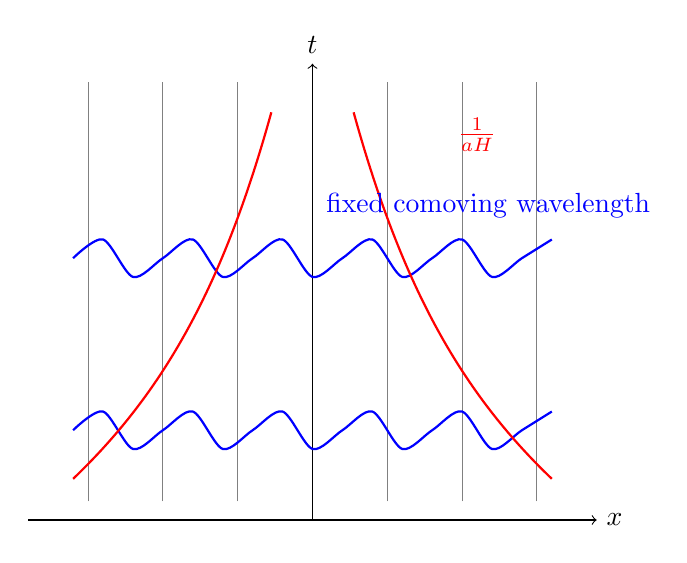
\begin{tikzpicture}[scale=0.95]
\draw[->] (-3.8,0) -- (3.8,0) node[right] {\(x\)};
\draw[->] (0,0) -- (0,6.1) node[above] {\(t\)};
\foreach \x in {-3,-2,-1,1,2,3}
  \draw[gray] (\x,0.25) -- (\x,5.85);
\draw[thick,blue] plot[smooth] coordinates {
(-3.2,1.2) (-2.8,1.45) (-2.4,0.95) (-2.0,1.2) (-1.6,1.45)
(-1.2,0.95) (-0.8,1.2) (-0.4,1.45) (0.0,0.95) (0.4,1.2)
(0.8,1.45) (1.2,0.95) (1.6,1.2) (2.0,1.45) (2.4,0.95)
(2.8,1.2) (3.2,1.45)
};
\draw[thick,blue] plot[smooth] coordinates {
(-3.2,3.5) (-2.8,3.75) (-2.4,3.25) (-2.0,3.5) (-1.6,3.75)
(-1.2,3.25) (-0.8,3.5) (-0.4,3.75) (0.0,3.25) (0.4,3.5)
(0.8,3.75) (1.2,3.25) (1.6,3.5) (2.0,3.75) (2.4,3.25)
(2.8,3.5) (3.2,3.75)
};
\draw[red,thick] (-3.2,0.55) .. controls (-2.0,1.7) and (-1.2,3.1) .. (-0.55,5.45);
\draw[red,thick] (3.2,0.55) .. controls (2.0,1.7) and (1.2,3.1) .. (0.55,5.45);
\node[blue] at (2.35,4.2) {fixed comoving wavelength};
\node[red] at (2.2,5.15) {\(\frac{1}{aH}\)};
\end{tikzpicture}
\caption{A spacetime sketch in comoving coordinates. The mode keeps roughly the same coordinate wavelength while the comoving horizon shrinks. Once the mode extends beyond the horizon, it freezes.}
\end{figure}

The lecture explains freeze-out with a rope analogy. A wave oscillates because each segment is pulled by neighboring segments. But if the wavelength is larger than the horizon, the relevant neighbors are causally inaccessible. The restoring pull is lost. Thus a mode ceases to oscillate when its physical wavelength exceeds the horizon size:
\begin{equation}
\lambda_{\rm phys}\gtrsim H^{-1}
\qquad \Longrightarrow \qquad
\text{freeze-out}.
\end{equation}

This happens mode by mode. Longer wavelengths freeze first, shorter wavelengths later, but in an exponentially expanding universe every mode is eventually stretched beyond the horizon. The fluctuations do not disappear; rather, they become frozen classical-looking variations of the field.

That is not the end of the story. The process continues. New vacuum fluctuations are constantly being produced on short scales; then expansion stretches them; then they freeze. At any given comoving point the field executes a random walk as one frozen mode after another is added with a random phase. Across space, different points undergo different random walks. This is what produces a statistical field of perturbations.

Because the same mechanism repeats on each logarithmic scale, the spectrum is approximately scale invariant. The lecture does not derive the exact power spectrum formula, and we should not smuggle it in here. What is secure is the qualitative claim: the frozen fluctuations look roughly similar from one scale to the next, with only small deviations from exact scale invariance.

When inflation ends, the horizon behavior changes. The horizon grows, and modes that had gone outside during inflation re-enter later. Once back inside the horizon they can evolve dynamically again. By then, however, they have been stretched to macroscopic scales, and the frozen field variations are converted into real density perturbations in the post-inflationary universe.

\subsection{Question \& Answer}

\paragraph{If inflation smooths everything out, why aren't the galaxy seeds erased?}

Because inflation smooths away preexisting classical irregularities, but it does not eliminate quantum zero-point fluctuations. On the contrary, as the universe expands, those quantum fluctuations are stretched beyond the horizon and freeze into real field variations. Inflation therefore erases the old roughness and manufactures a new one. The galaxy seeds are not leftover classical dirt; they are fossilized quantum fluctuations.

\section{What Inflation Predicts, What It Hides, and Why Fine-Tuning Returns}

The lecture's final move is to turn mechanism into prediction. Once the field has frozen-in fluctuations, neighboring regions do not all reach the cliff edge at the same time. A region that is slightly farther downhill falls first. Its vacuum energy is converted into radiation earlier, and that radiation then dilutes under expansion:
\begin{equation}
\rho_r\propto a^{-4}.
\end{equation}
A neighboring region still on the plateau remains vacuum dominated and does not dilute. When it falls later, it emerges with a larger post-inflation energy density. In this way small variations in \(\phi\) are converted into variations in density.

The lecture's qualitative scaling can be summarized schematically as
\begin{equation}
\delta t \sim \frac{\delta\phi}{\dot\phi},
\qquad
\frac{\delta\rho}{\rho}\propto H\,\delta t
\sim H\,\frac{\delta\phi}{\dot\phi}.
\end{equation}
This is not presented in the lecture as a formal derived formula, so it should be read only as a compact version of the spoken argument. Its meaning is the same as Susskind's: the smaller the terminal velocity \(\dot\phi\), the larger the final density contrast. Therefore flatter potentials produce larger fluctuations. Higher potentials also produce larger fluctuations. The width of the plateau mostly controls how long inflation lasts, that is, how many e-foldings occur.

The lecture then turns to gravitational waves. If the inflationary energy scale is high enough, tensor fluctuations should also be produced. The absence of a large gravitational-wave contribution already tells us that the scale cannot be too high; if it is too low, there is no realistic hope of seeing the tensor signal. The numerical bounds are given only as ballpark figures, and should remain that way here. In Planck units the relevant energy density is something like \(10^{-14}\) to \(10^{-16}\), with the important point being that the observable window is narrow.

To make sense of those numbers, the lecture pauses over units. In natural units with \(c=\hbar=1\), mass has the dimensions of inverse length, so an energy density has dimensions
\begin{equation}
[\rho]=(\text{mass})^4.
\end{equation}
Thus statements such as \(V\sim 10^{-14}\) or \(V\sim 10^{-123}\) in Planck units mean that the energy density has been measured relative to \(M_{\rm Pl}^4\).

The next point is subtler. Inflation is successful precisely because it washes out what came before. That is its virtue. But it is also its vice. If inflation lasts long enough, the earlier history becomes practically inaccessible, because the later quantum fluctuations dominate what we can observe. The lecture treats this as a double-edged conclusion: inflation correlates data on widely separated scales with impressive success, yet the same success makes the pre-inflationary past hard to reconstruct.

A late caveat is then added. Pure de Sitter expansion is often described by \(a(t)\propto e^{Ht}\), but that is only the late-time behavior in a particular slicing. The global de Sitter solution is more accurately represented by
\begin{equation}
a(t)\propto \cosh(Ht),
\end{equation}
which contracts to a minimum size and then re-expands. The lecture leaves open whether the contracting branch should be taken literally in cosmology. The point is not to settle that issue, but to remind us that even the simplest inflationary geometry has interpretive subtleties.

The final discussion ties inflation back to fine-tuning and structure formation. There are, in the lecture's language, two puzzles. One is the required flatness of the inflationary potential, which he characterizes as a mild tuning, of order a few percent, if one asks for enough e-foldings directly from the parameter space of the model. The other is the cosmological constant today, of order \(10^{-123}\), which looks fantastically small.

The lecture then offers the anthropic turn. A positive cosmological constant acts, in Newtonian language, like a repulsion proportional to distance. If it were only a couple of orders of magnitude larger than the observed value, it would not necessarily rip apart galaxies that already existed, but it would prevent the primordial \(10^{-5}\) fluctuations from ever condensing into galaxies in the first place. This is the content of Weinberg's argument: the cosmological constant need not be exactly zero; it need only be small enough that structure can form.

Negative curvature creates a parallel problem. Too much outward recession, in excess of the effective escape condition, also prevents collapse. Inflation dilutes curvature. Asking how much inflation is needed therefore becomes another structure-formation question. The lecture quotes about \(59.5\) e-foldings as the minimum needed so that curvature does not obstruct galaxy formation, with a benchmark of roughly \(62\) e-foldings as the empirically relevant figure for our universe.

This changes the probability question. If one asks for the raw fraction of parameter space that gives sufficient inflation, the answer may be small, on the order of a few percent. But if one conditions on the existence of observers in a universe with galaxies, then the region with too few e-foldings or too large a cosmological constant is simply discarded, and the conditional probability can become large. The lecture does not present this as a final solution. It presents it as the place where the great puzzles and the great debates now live.

\section{Summary}

The lecture begins with \(\Omega\), because before inflation can explain anything it must answer to observation. The observed universe is nearly flat, and in the late universe that means the normalized matter and vacuum contributions nearly saturate the Friedmann equation. Inflation is then introduced as the mechanism that makes the universe so large and so smooth; structure formation reintroduces the need for small primordial irregularities; pressure delays collapse until matter domination; dark matter starts the process early; a scalar field on a shallow potential sustains inflation; Hubble friction makes slow roll possible; quantum fluctuations freeze beyond the horizon and seed later structure; and the final successes of the theory return us to fine-tuning, anthropic reasoning, and the unsettling fact that inflation explains the observable universe partly by erasing what came before it.